Parallel programming model is a set of software technologies to express parallel algorithms and match applications with the underlying parallel systems. \hypertarget{_parallel_programming_model_ParallelProgrammingModelSerialComputingvsParallelComputing}{}\section{Serial Computing vs Parallel Computing}\label{_parallel_programming_model_ParallelProgrammingModelSerialComputingvsParallelComputing}
\begin{TabularC}{2}
\hline
\rowcolor{lightgray}{\bf Serial Computing }&{\bf Parallel Computing  }\\\cline{1-2}
A problem is broken into a discrete series of instructions &A problem is broken into discrete parts that can be solved concurrently \\\cline{1-2}
Instructions are executed sequentially one after another &Each part is further broken down to a series of instructions \\\cline{1-2}
Executed on a single processor &Instructions from each part execute simultaneously on different processors \\\cline{1-2}
Only one instruction may execute at any moment in time &An overall control/coordination mechanism is employed \\\cline{1-2}
\end{TabularC}
\hypertarget{_parallel_programming_model_ParallelProgrammingModelSerialComputingvsParallelComputingSerialComputingDiagram}{}\subsection{Serial Computing Diagram}\label{_parallel_programming_model_ParallelProgrammingModelSerialComputingvsParallelComputingSerialComputingDiagram}

\begin{DoxyImageNoCaption}
  \mbox{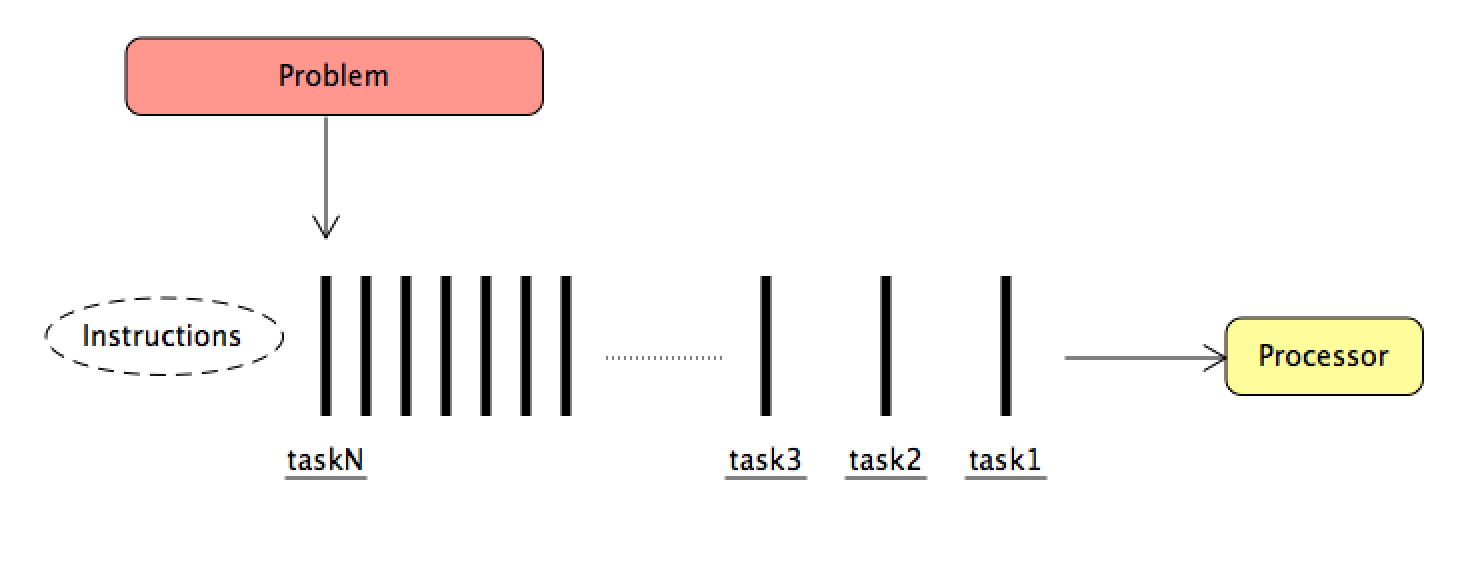
\includegraphics[width=\textwidth,height=\textheight/2,keepaspectratio=true]{ResearchSerialComputingDiagram.png}}
\end{DoxyImageNoCaption}
 \hypertarget{_parallel_programming_model_ParallelProgrammingModelSerialComputingvsParallelComputingParallelComputingDiagram}{}\subsection{Parallel Computing Diagram}\label{_parallel_programming_model_ParallelProgrammingModelSerialComputingvsParallelComputingParallelComputingDiagram}

\begin{DoxyImageNoCaption}
  \mbox{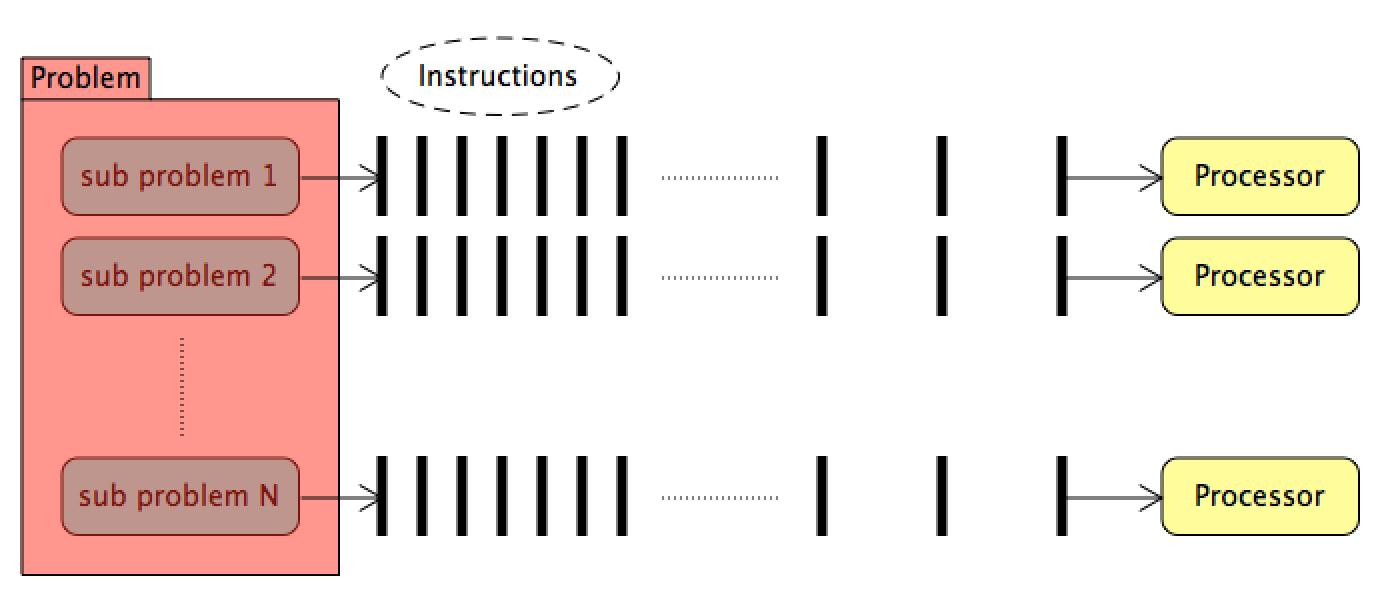
\includegraphics[width=\textwidth,height=\textheight/2,keepaspectratio=true]{ResearchParallelComputingDiagram.png}}
\end{DoxyImageNoCaption}
\hypertarget{_parallel_programming_model_ParallelProgrammingModelOpenMP}{}\section{Open\+M\+P}\label{_parallel_programming_model_ParallelProgrammingModelOpenMP}
The Open Multi-\/\+Processing (Open\+M\+P) is a library that can be used to specify shared memory parallelism in Fortran and C/\+C++ programs. It provides a model for parallel programming that is portable across shared memory architectures from different vendors. The benefit of Open\+M\+P is it is very easy. Open\+M\+P is compiler directive based that means to use Open\+M\+P you need a open\+M\+P supported Compiler.\+More information about the Open\+M\+P A\+P\+I can be found at \href{http://www.openmp.org}{\tt http\+://www.\+openmp.\+org}.\hypertarget{_parallel_programming_model_ParallelProgrammingModelIntelTBB}{}\section{Intel T\+B\+B}\label{_parallel_programming_model_ParallelProgrammingModelIntelTBB}
Intel Threading Building Blocks (Intel T\+B\+B) is a C and C++ library for creating high performance and scalable parallel applications. It provides a set of interfaces, functions, and renders for implementing parallelism. The advantage of Intel T\+B\+B is it is not compiler directive based as Open\+M\+P that means you can use whatever compiler you preferred.\hypertarget{_parallel_programming_model_ParallelProgrammingModelConcurrencyModel}{}\section{Concurrency Model}\label{_parallel_programming_model_ParallelProgrammingModelConcurrencyModel}
Concurrency is a property of systems in which several computations are executing simultaneously, and potentially interacting with each other. ~\newline
~\newline
Concurrency vs Parallelism \cite{parallelismVsConcurrency} \begin{TabularC}{2}
\hline
\rowcolor{lightgray}{\bf Concurrency }&{\bf Parallelism  }\\\cline{1-2}
Concurrency is when two tasks can start, run, and complete in overlapping time periods. It doesn\textquotesingle{}t necessarily mean they\textquotesingle{}ll ever both be running at the same instant. Eg. multitasking on a single-\/core machine. &Parallelism is when tasks literally run at the same time. Eg. on a multicore processor. \\\cline{1-2}
Eg. multitasking on a single-\/core machine. &Eg. on a multicore processor. \\\cline{1-2}
A condition that exists when at least two threads are making progress. A more generalized form of parallelism that can include time-\/slicing as a form of virtual parallelism. &A condition that arises when at least two threads are executing simultaneously. \\\cline{1-2}
\end{TabularC}
~\newline
~\newline
Example Concurrency Models\+:
\begin{DoxyItemize}
\item Actors Model
\item C\+S\+P (Communicating Sequential Processes)
\item Disruptor
\item Thread 
\end{DoxyItemize}